\documentclass[12pt]{article}  
\usepackage{graphicx}
\usepackage{t1enc}
\usepackage{bm}
\usepackage{url}
\usepackage{amsmath}
\usepackage{algorithm}
\usepackage{algpseudocode}
\usepackage{tikz}
\usetikzlibrary{shapes.geometric, arrows}
\usetikzlibrary{positioning,arrows}

\tikzstyle{process} = [rectangle, rounded corners, minimum height=1cm, text centered, text width=2cm, draw=black, font=\scriptsize]
\tikzstyle{state} = [ellipse, minimum height=1cm, text centered, text width=1.5cm, draw=black, font=\scriptsize]
\tikzstyle{description} = [rectangle, minimum height=1.5cm, text centered, text width=3.5cm, draw=black, font=\scriptsize]

\tikzstyle{arrow} = [thick,->,>=stealth]
\tikzstyle{line} = [thick,--,>=stealth]

\def\ex#1{\hbox{\tt #1}}

\date{}
\begin{document}
\begin{center}\Large
        CMPUT 551 --- Project Report\\
        Sentiment Analysis in Figurative Language\\
        \tiny (Using Twitter Data)\\
        \vspace{0.30in}
        \small
        \begin{tabular}{@{}ll}
        Adam St. Arnaud &-~~ ajstarna@ualberta.ca\\
        Alexandr Petcovici &-~~ apetcovi@ualberta.ca\\
        Janek Goergens &-~~ gorgens@ualberta.ca\\
        Robert Post &-~~ rpost@ualberta.ca\\
        Sankalp Prabhakar &-~~ sankalp@ualberta.ca\\
        \end{tabular}
        
\end{center}
\begin{tabular}{@{}ll}
Instructor: & Prof. R. Greiner \\
Supervisor: & Dr. Greg Kondrak\\
Date: & Friday, 12/Dec/2014
\end{tabular}


\hrule\hrule

\vspace{0.20in}
\tableofcontents


\newpage
\section{Introduction} % (fold)
\label{sec:introduction}
%!TEX root = ../report.tex
\subsection{The Problem} % (fold)
\label{sub:the_problem}
Sentiment analysis is the area of natural language processing (NLP) concerned with computationally identifying the emotion expressed by an author of a piece of text (positive, negative, neutral). Determining the sentiment of a piece of text has important implications for opinion mining, parsing users reviews and recommendation systems. Humans communicate in complicated ways and often don't strictly use literal language. Figurative language, such as sarcasm, irony, and metaphors, are quite prevalent in standard human communication. Hence, in order to create better representations of human language, systems must take figurative language into account.
% subsection the_problem (end)

\subsection{Related Work} % (fold)
\label{sub:related_work}

% subsection related_work (end)

\subsection{Motivation} % (fold)
\label{sub:motivation}

% subsection motivation (end)
% section introduction (end)

\newpage
\section{Problem Formulation} % (fold)
\label{sec:problem_formulation}
%!TEX root = ../report.tex
\subsection{Twitter Data} % (fold)
\label{sub:twitter_data}
Twitter is a web platform where users can post short messages with up to 140 characters to broadcast things they want the world to know. These messages are called \textit{tweets} and the whole Twitter system became very famous in the last years. That's the reason why there's a high interest in performing sentiment analysis on twitter data. We are provided with a set of 8000 tweets where each tweet was annotaded by 7 persons. Each one scored the given tweet on a range from $-5$ to $5$ (where $-5$ indicates a very negativ, $0$ a neutral and $5$ a positive sentiment). The highest and lowest rate were ignored and the average of the remaining 5 scores is given for every 8000 tweets. This data is provided by \textit{SemEval-2015 Task 11}.
% subsection twitter_data (end)

\subsection{Histogram} % (fold)
\label{sub:histogram}
In figure \ref{fig:hist_data} you can see, that the most tweets have a score next to negative 2

\begin{figure}[ht]
\centering 
  \begin{tabular}{@{}l@{}}
    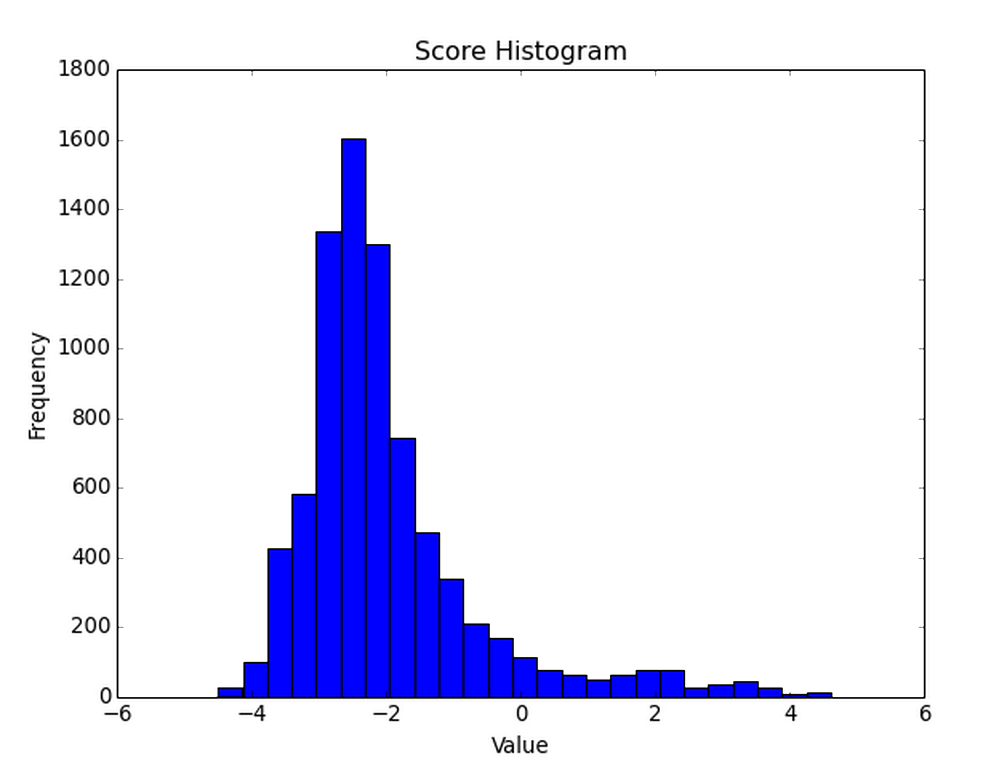
\includegraphics[width=0.6\linewidth]{img/data_hist.png}
  \end{tabular} 
  \caption{Histogram showing the score distribution for the given data} 
  \label{fig:hist_data} 
\end{figure}

% subsection histogram (end)

\subsection{Learning Task} % (fold)
\label{sub:learning_task}
yes
% subsection learning_task (end)

\subsection{Pipeline} % (fold)
\label{sub:pipeline}

% subsection pipeline (end)

\subsection{Evaluation} % (fold)
\label{sub:evaluation}

% subsection evaluation (end)
% section problem_formulation (end)

\newpage
\section{Preprocessing} % (fold)
\label{sec:preprocessing}
%!TEX root = ../report_nips.tex
\subsection{pp1} % (fold)
\label{sub:pp1}

Lorem ipsum dolor sit amet, consectetur adipisicing elit, sed do eiusmod
tempor incididunt ut labore et dolore magna aliqua. Ut enim ad minim veniam,
quis nostrud exercitation ullamco laboris nisi ut aliquip ex ea commodo
consequat. Duis aute irure dolor in reprehenderit in voluptate velit esse
cillum dolore eu fugiat nulla pariatur. Excepteur sint occaecat cupidatat non
proident, sunt in culpa qui officia deserunt mollit anim id est laborum.

\begin{table}[t]
\caption{Sample table title}
\label{sample-table}
\begin{center}
\begin{tabular}{l | L{4cm} | L{2cm} | L{2cm} | l}
\multicolumn{1}{c}{\bf NAME}  &\multicolumn{1}{c}{\bf DEFINITION} &\multicolumn{2}{c}{\bf EXAMPLE} &\multicolumn{1}{c}{\bf UNIQUE TOKENS}\\
\multicolumn{2}{c}{}  &\multicolumn{1}{c}{\tiny BEFORE} &\multicolumn{1}{c}{\tiny AFTER} &\multicolumn{1}{c}{\bf COUNT}
\\ \hline 

Convert to lowercase &
Converts all characters from a word to lowercase &
PLEASE &
please &
20092 \\ \hline

\multirow{5}{*}{Remove apostrophe} &
\multirow{2}{4cm}{Removes apostrophe and return the original words for most common cases where apostrophe is used as vowel substitution} &
you're &
you are &
\multirow{5}{*}{22718} \\[.6cm]
&&I've & I have & \\[.6cm] \hline


De-elongate words &
Convert elongated words to normal version (works in combination with automated grammar corrector &
pleeeeeeese &
pleease (please – after grammar corrector) &
22640 \\ \hline


\multirow{9}{*}{Remove stop words} &
\multirow{3}{4cm}{There does not exist a single definition of stop words. For our task stop words are words which do not have any sentimental load. We used the stop word list from nltk corpus except words “no” and “not”
under} &
under & &
\multirow{9}{*}{22640}\\[.4cm]
&&before&&\\[.4cm]
&&very&&\\[.4cm]
&&to&&\\[.4cm] \hline



\end{tabular}
\end{center}
\end{table}


% subsection pp1 (end)

\subsection{pp2} % (fold)
\label{sub:pp2}

% subsection pp2 (end)
% section preprocessing (end)

\newpage
\section{Features} % (fold)
\label{sec:features}
%!TEX root = ../report.tex
\subsection{n-Grams} % (fold)
\label{sub:n_grams}

% subsection n_grams (end)

\subsection{Part of Speec (POS) Tagging} % (fold)
\label{sub:part_of_speec_}

One of the most fundamental parts of the linguistic pipeline is the part-of-speech (POS) tagging, a basic form of syntactic analysis which has countless applications in Natural Language Processing (NLP). We studied some of the best POS tagging tools \& settled on using Tweet NLP, a twitter specific POS tagger. We’ve used part-of-speech tagging as a feature for our task wherein every word/token in a given tweet is tagged based on its part-of-speech, some of which are twitter specific.

For our task, we selected 15 of the most common tags in linguistics (including the twitter specific tags). we made a count of the number of tagged tokens (with a confidence score > 0.9) in a tweet \& then used that as a feature.[rough work]

% subsection part_of_speec_ (end)

\subsection{Sentiment} % (fold)
\label{sub:sentiment}

We used \textit{SentiWordNet} to add features specifically related to the sentiment of the tweets. This is dictionary, designed for opinion mining, where each of the over 100,000 words is assigned a positive and negative sentiment score. For a given tweet, we calculate a positive sum feature: $p_{sum} = \sum_{i}^n p_i$ , where piis the positive sentiment score from SentiWordNet for the ith word in a tweet with n words. We similarly calculate a negative sum feature. If a word is not found in the dictionary, then it does not contribute to either of the two sentiment features. These two features are added to the bag of words feature vector as a real number. It is possible that different preprocessing steps could affect the sentiment score of a tweet by modifying said tweet (such as by stemming); future experimentation is required to determine the effects of different combinations of preprocessing on sentiment score.

% subsection sentiment (end)

\subsection{Irony} % (fold)
\label{sub:irony}

To account for possible irony in the tweets we implement two features based on the work of Reyes et. al [year]. The features are created to detect the so-called \textit{counter-factuality} and \textit{temporal compression} of a tweet. Reyes et. al. determined that ironic tweets were more likely to have a high level of these two measures.

\paragraph{Counter-factuality:} % (fold)
\label{par:counter_factuality_}
The first measure, counter-factuality, is focused on ``discursive terms that hint at opposition or contradiction in a text, such as about, nevertheless, nonetheless, and yet.'' (Citation). The full list of counter-factual words includes 41 entrees; there are a total of 4187 occurrences of these words in the data set, and 3123 tweets contain at least one counter-factual word.
% paragraph counter_factuality_ (end)

\paragraph{Temporal Compression:} % (fold)
\label{par:temporal_compression_}
The second measure of tweet irony that we considered is temporal compression, which focuses on words related to an opposition in time, thus indicating an abrupt change in narrative. (citation) The list of temporal compression words contains 13 words such as suddenly, abruptly, and now. There are only 170 instances of a temporal compression word in the dataset, with only 103 tweets even containing a single instance.
% paragraph temporal_compression_ (end)

\paragraph{Feature Creation:} % (fold)
\label{par:feature_creation_}
For each measure, we create a real-numbered feature based on the ratio of how many words in a given tweet possess the characteristic we are analyzing. That is, we have two ratio features $r_t = \frac{n_t}{n}$, where $t \in \left \{\ex{counterFactuality}, \ex{temporalCompression}\right \}$, $n_t$ is the number of words in a given tweet that fit into category $t$, and $n$ is the total number of words in the tweet.
% paragraph feature_creation_ (end)

% subsection irony (end)
% section features (end)

\newpage
\section{Experiments / Results} % (fold)
\label{sec:experiments_results}
%!TEX root = ../report.tex
\subsection{Experiment 1} % (fold)
\label{sub:experiment_1}

% subsection experiment_1 (end)

\subsection{Experiment 2} % (fold)
\label{sub:experiment_2}

% subsection experiment_2 (end)
% section experiments_results (end)

\newpage
\section{Conclusion} % (fold)
\label{sec:conclusion}
%!TEX root = ../report.tex
% section conclusion (end)
\end{document}